\documentclass[11pt,a4paper, twoside]{report}
\usepackage[margin=1in, headheight=14pt]{geometry}
\usepackage{amsfonts,amsmath,amssymb,suetterl}
\usepackage{lmodern}
\usepackage[T1]{fontenc}
\usepackage{fancyhdr}
\usepackage{float}
\usepackage[utf8]{inputenc}
\usepackage{fontawesome}
\usepackage{enumerate}
\usepackage{xcolor}
\usepackage{hyperref}
\usepackage{tikz}
\usepackage{nicefrac}
\usepackage{subcaption}
\usepackage{physics}
\usepackage{mathtools}
\usepackage{adjustbox}

\DeclareUnicodeCharacter{2212}{-}

\usepackage{mathrsfs}
\usepackage[nodisplayskipstretch]{setspace}

\setstretch{1.5}
\renewcommand{\footrulewidth}{0pt}

\pagestyle{fancy}
\fancyhead[RO]{PARTIAL DIFFERENTIAL EQUATIONS}
\fancyhead[LE]{THE METHOD OF SEPARATION OF VARIABLES}

\parindent 0ex
\setlength{\parskip}{1em}
\raggedbottom

\begin{document}
	\textbf{B. Example: The Vibrating String Problem}\par
	We now illustrate the method of separation of variables by applying it to obtain a formal solution of the so-called vibrating string problem.\par
	\textbf{The Physical Problem.} Consider a tightly stretched elastic string the ends of which are fixed on the $x$ axis at $x = 0$ and $x = L$. Suppose that for each $x$ in the interval $0 < x < L$ the string is displaced into the my plane and that for each such $x$ the displacement from the $x$ axis is given by $f(x)$, where $f$ is a known function of $x$ (see Figure 14.1).
	%
	\begin{figure}[H]
		\centering
		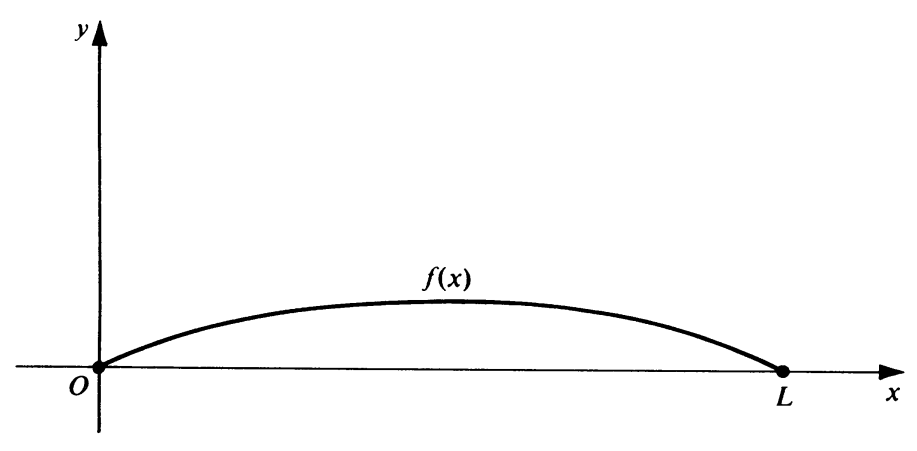
\includegraphics[width=0.75\textwidth]{figure/1_page_1.PNG}
		\caption*{Figure 14.1}
	\end{figure}
	%
	Suppose that at $x = 0$ the string is released from the initial position defined by $f(x)$, with an initial velocity given at each point of the interval $0 \leq x \leq L$ by $g(x)$, where $g$ is a known function of $x$. Obviously the string will vibrate, and its displacement in the $y$ direction at any point $x$ at any time $t$ will be a function of both $x$ and $t$. We seek to find this displacement as a function of $x$ and $t$; we denote it by $y$ or $y(x, t)$.\\
	We now make certain assumptions concerning the string, its vibrations, and its  surroundings. To begin with, we assume that the string is perfectly flexible, is of  constant linear density $\rho$, and is of constant tension $T$ at all times. Concerning the vibrations, we assume that the motion is confined to the $xy$ plane and that each point on the string moves on a straight line perpendicular to the $x$. axis as the string vibrates. Further, we assume that the displacement $y$ at each point of the string is small compared to the length length $L$ and that the angle between the string and the the $x$ axis at each point is also sufficiently small. Finally, we assume that no external forces (such as damping forces, for example) act upon the string.\\
	Although these assumptions are not actually valid in any physical problem, nevertheless they are approximately satisfied in many cases. They are made in order to make the  resulting mathematical problem more tractable. With these assumptions, then, the problem is to find the displacement $y$ as a function of $x$ and $t$.\par
	\textbf{The Mathematical Problem.} Under the assumptions stated it can be shown that the displacement $y$ satisfies the partial differential equation,
	%
	\begin{equation}\tag{14.20}\label{14.20}
		\alpha^2 \frac{\partial^2 y}{\partial x^2} = \frac{\partial^2 y}{\partial t^2}
	\end{equation}


	where $\alpha^2 = T/\rho$. This is the one-dimensional wave equation, a special case of which we have already studied in Example 14.3. Since our primary concern here is to illustrate the method of separation of variables, we omit the derivation of the equation.\\
	Since the ends of the string are fixed at $x = 0$ and $x = L$ for all time $t$, the displacement $y$ must satisfy the boundary conditions
	%
	\begin{equation}\tag{14.21}\label{14.21}
		\begin{aligned}
			y(0, t) = 0, \quad 0 \leq t < \infty;\\
			y(L, t) = 0,\quad 0 \leq t < \infty.
		\end{aligned}
	\end{equation}
	At $t = 0$ the string is released from the initial position defined by $f(x),\ 0 \leq x \leq L$, with initial velocity given by $g(x),\ 0 \leq x \leq L$. Thus the displacement $y$ must also satisfy the initial conditions
	%
	\begin{equation}\tag{14.22}\label{14.22}
		\begin{aligned}
			y(x, 0) &= f(x),\quad 0 \leq x \leq;\\
			\frac{\partial y(x, 0)}{\partial t} = g(x),\quad 0 \leq x \leq L.
		\end{aligned}
	\end{equation}
	This, then, is our problem. We must find a function $y$ of $x$ and $t$ which satisfies the partial differential equation (14.20), the boundary conditions (14.21), and the initial conditions (14.22).\par
	\textbf{Solution} We apply the method of separation of variables. We first make the basic assumption that the differential equation (14.20) has product solutions of the form $XT$, where $X$ is a function of $x$ only and $T$ is a function of $t$ only. To emphasize this, we write
	%
	\begin{equation}\tag{14.23}\label{14.23}
		y(x, t) = X(x)T(t)
	\end{equation}
	We now differentiate (14.23) and substitute into the differential equation (14.20). Differentiating, we find
	$$
	\frac{\partial^2 y}{\partial x^2} = T\frac{d^2 X}{dx^2}\quad \text{and}\quad \frac{\partial^2 y}{\partial t^2} = X\frac{d^2 T}{dt^2}
	$$
	substituting, we obtain
	$$
	\alpha^2 T\frac{d^2 X}{dx^2} = X \frac{d^2 T}{dt^2}.
	$$
	From this we obtain at once
	%
	\begin{equation}\tag{14.24}\label{14.24}
		\alpha^2 \frac{\frac{d^2 T}{dx^2}}{X} = \frac{\frac{d^2T}{dt^2}}{T}.
	\end{equation}
	Since $X$ is a function of $x$ only, the left member of (14.24) is also a function of $x$ only and hence is independent of $t$. Further, since $T$ is a function of $t$ only, the right member of (14.24) is also a function of $t$ only and hence is independent of $x$. Since one of the two equal expressions in (14.24) is independent of $t$ and the other one is independent of $x$, both of them must be equal to a constant $k$. That is, we have
	$$
	\alpha^2 \frac{\frac{d^2 X}{dx^2}}{X} = k\quad \text{and}\quad \frac{\frac{d^2T}{dt^2}}{T} = k.
	$$
	From this we obtain the two ordinary differential equations
	%
	\begin{equation}\tag{14.25}\label{14.25}
		\frac{d^2 X}{dx^2} - \frac{k}{\alpha^2}X = 0
	\end{equation}
	and
	%
	\begin{equation}\tag{14.26}\label{14.26}
		\frac{d^2 T}{dt^2} - kT = 0.
	\end{equation}
	Let us now consider the boundary conditions (14.21). Since $y(x, t) = X(x)T(t)$, we see that $y(0, t) = X(0)T(t)$ and $y(L, t) = X(L)T(t)$. Thus the boundary conditions (14.21) take the forms
	%
	\begin{equation*}
		\begin{aligned}
			X(0)T(t) = 0,\quad 0 \leq t < \infty;\\
			X(L)T(t) = 0, \quad 0 \leq t < \infty.
		\end{aligned}
	\end{equation*}
	Since $T(t) = 0,\ 0 \leq t < \infty$, would reduce the assumed solution (14.23) to the trivial solution of (14.20), we must have
	%
	\begin{equation}\tag{14.27}\label{14.27}
		X(0) = 0\quad \text{and}\quad X(L) = 0.
	\end{equation}
	Thus the function $X$ in the assumed solution (14.23) must satisfy both the ordinary differential equation (14.25) and the boundary conditions (14.27). That is, the function $X$ must be a nontrivial solution of the Sturm-Liouville problem
	%
	\begin{equation}\tag{14.25}
		\frac{d^2X}{dx^2} - \frac{k}{\alpha^2}X = 0,
	\end{equation}
	%
	\begin{equation}\tag{14.27}
		X(0) = 0,\quad X(L) = 0.
	\end{equation}
	We have already solved a special case of this problem in Example 12.3 of Chapter 12. Our procedure here will parallel the treatment in that example. We must first find the general solution of the differential equation (14.25). The form of this general solution depends upon whether $k = 0,\ k > 0$, or $k < 0$.\\
	If $k = 0$ the general solution of (14.25) is of the form
	%
	\begin{equation}\tag{14.28}\label{14.28}
		X = c_1 + c_2x.
	\end{equation}
	We apply the boundary conditions (14.27) to the solution (14.28). The condition $X(0) = 0$ requires that $c_1 - 0$. The condition $X(L) = 0$ becomes $c_1 + c_2L = 0$. Since $c_1 = 0$, this requires that $c_2 = 0$ also. Thus the solution (14.28) reduces to the trivial solution.\\
	IF $k>0$, the general solution of (14.25) is of the form
	%
	\begin{equation}\tag{14.29}\label{14.29}
		X = c_1e^{\sqrt{k}x/\alpha} + c_2e^{-\sqrt{k}x/\alpha}.
	\end{equation}
	Applying the boundary conditions (14.27) to the solution (14.29), we obtain the system of equations
	%
	\begin{equation}\tag{14.30}\label{14.30}
		\begin{aligned}
			c_1 + c_2 = 0,\\
			c_1e^{\sqrt{k}L/\alpha} + c_2e^{-\sqrt{k}L/\alpha}.
		\end{aligned}
	\end{equation}
	To obtain nontrivial solutions of this system, we must have
	$$
	\begin{vmatrix}
		1 & 1\\
		e^{\sqrt{k}L/\alpha} & e^{-\sqrt{k}L/\alpha}
	\end{vmatrix} = 0.
	$$
	But this implies that $e^{\sqrt{k}L/\alpha}$ and hence that $k = 0$, contrary to our assumption in this case. Thus the system (14.30) has no nontrivial solutions, and so the solution (14.29) also reduces to the trivial solution.\\
	Finally, if $k<0$, the general solution of (14.25) is of the form
	%
	\begin{equation}\tag{14.31}\label{14.31}
		X = c_1 \sin \frac{\sqrt{-k}x}{\alpha} + c_2 \cos \frac{\sqrt{-k}x}{\alpha}.
	\end{equation}
	Applying the boundary conditions (14.27) to the solution (14.31), we obtain
	$$
	c = 0
	$$
	and
	$$
	c_1 \sin \frac{\sqrt{-k}L}{\alpha} + c_2 \cos \frac{\sqrt{-k}L}{\alpha} = 0
	$$
	Since $c_2 = 0$, the latter condition reduces to
	$$
	c_1 \sin \frac{\sqrt{-k}L}{\alpha} = 0.
	$$
	Thus to obtain nontrivial solutions of the form (14.31), we must have
	$$
	\frac{\sqrt{-k}L}{\alpha} = n\pi \quad (n = 1,\ 2,\ 3,\ \ldots),
	$$
	and so
	\begin{equation}\tag{14.32}\label{14.32}
		k = -\frac{n^2\pi^2\alpha^2}{L^2}\quad (n = 1,\ 2,\ 3,\ \ldots)
	\end{equation}
	We thus find that the constant $k$ must be a negative number of the form (14.32). We recognize these values of $k$ as the characteristic values of the Sturm—Liouville problem under consideration. The corresponding nontrivial solutions (the characteristic functions) of the problem are then
	%
	\begin{equation}\tag{14.33}\label{14.33}
		X_n - c_n \sin \frac{n\pi x}{L}\quad (n = 1,\ 2,\ 3,\ \ldots),
	\end{equation}
	where the $c_n(n = 1,\ 2,\ 3,\ \ldots)$are arbitrary constants. We thus find that the function $X$ in the assumed solution (14.23) must be of the form (14.33). That is, corresponding to each positive integral value of $n$, we obtain functions $X_n$ of the form (14.33) which will serve as the function $X$ in the product solution (14.23).\\
	Let us now return to the differential equation (14.26) which the function F in (14.23) must satisfy. Since k must be of the form (14.32), the differential equation (14.26) becomes
	$$
	\frac{d^2 T}{dt^2} + \frac{n^2 \pi^2 \alpha^2}{L^2}T = 0,
	$$
	where $n = 1,\ 2,\ 3,\ \ldots$. For each such value of $n$, this differential equation has solutions of the form
	%
	\begin{equation}\tag{14.34}\label{14.34}
		T_n = c_{n, 1}\sin \frac{n \pi \alpha t}{L} + c_{n, 2}\cos \frac{n \pi \alpha t}{L}\quad (n = 1,\ 2,\ 3,\ \ldots),
	\end{equation}
	where the $c_{n, 1}$ and $c_{n, 2}(n = 1, 2, 3,\ldots)$ are arbitrary constants. Thus the function $T$ in the assumed solution (14.23) must be of the form (14.34). That is, corresponding to each positive integral value of $n$, we obtain functions $T_n$ of the form (14.34) which will serve as the function $T$ the product solution (14.23).\\
	Therefore, corresponding to each positive integral value of value of $n(n = 1,\ 2,\ 3,\ \ldots)$, we obtain solutions
	$$
	X_nT_n = \left[c_n\sin \frac{n \pi x}{L}\right]\left[c_{n,1}\sin \frac{n\pi \alpha t}{L} + c_{n, 2}\cos \frac{n\pi \alpha t}{L}\right]
	$$
	which have the product form (14.23).\\
	We set $a_n = c_nc_{n,1}$ and $b_n = c_nc_{n,2}(n = 1,\ 2,\ 3,\ \ldots)$ and write these solutions as
	%
	\begin{equation}\tag{14.35}\label{14.35}
		y_n(x, t) = \left[\sin \frac{n\pi x}{L}\right]\left[a_n\sin \frac{n\pi \alpha t}{L} + b_n \cos \frac{n \pi \alpha t}{L}\right]\quad (n=1,\ 2,\ 3,\ \ldots)
	\end{equation}
	We point out that each of these solutions (14.35) satisfies both the partial differential equation (14.20) and the two boundary conditions (14.21) for all values of the constants $a_n$ and $b_n$.\\
	We must now try to satisfy the two initial conditions (14.22). In general no single one of the solutions (14.35) will satisfy these conditions. For example, if we apply the first initial condition (14.22) to a solution of the form (14.35) we must have
	$$
	b_n \sin \frac{n \pi x}{L} = L(x),\quad 0\leq x \leq L,
	$$
	where $n$ is some positive integer; and this is clearly impossible unless $f$ happens to be a sine function of the form $A\sin (n\pi x/L)$ for some positive integer $n$.\\
	What can we do now? By Theorem 14.1 every finite linear combination of solutions of (14.20) is also a solution of (14.20); and by Theorem 14.2, assuming appropriate convergence, an infinite series of solutions of (14.20) is also a solution of (14.20). This suggests that we should form either a finite linear combination or an infinite series of the solutions (14.35) and attempt to apply the initial conditions (14.22) to the “more general" solutions thus obtained. In general no finite linear combination will satisfy these conditions, and we must resort to an infinite series.\\
	We therefore form an infinite series
	$$
	\sum_{n=1}^\infty y_n(x,t) = \sum_{n=1}^\infty \left[\sin \frac{n \pi x}{L}\right]\left[a_n \sin\frac{n\pi\alpha t}{L} + b_n\cos \frac{n\pi \alpha t}{L}\right]
	$$
	of the solutions (14.35). Assuming appropriate convergence, Theorem 14.2 applies and assures us that the sum of this series is also a solution of the differential equation (14.20). Denoting this sum by $y(x, t)$, we write
	%
	\begin{equation}\tag{14.36}\label{14.36}
		y(x, t) = \sum_{n=1}^\infty\left[\sin \frac{n\pi x}{L}\right]\left[a_n\sin \frac{n\pi \alpha t}{L} + b_n\cos \frac{n \pi \alpha t}{L}\right],
	\end{equation}
	We note that $y(0, t) = 0$ and $y(L, t) = 0$. Thus, assuming appropriate convergence, the function $y$ given by (14.36) satisfies both the differential equation (14.20) and the two boundary conditions (14.21).\\
	Let us now apply the initial conditions (14.22) to the series solution (14.36). The first condition $y(x, 0) = f(x),\ 0 \leq x \leq L$, reduces (14.36) to
	%
	\begin{equation}\tag{14.37}\label{14.37}
		\sum_{n=1}^\infty b_n \sin \frac{n \pi x}{L} = f(x),\quad 0 \leq x \leq L.
	\end{equation}
	Thus to satisfy the first initial condition (14.22), we must determine the coefficients $b_n$ so that (14.37) is satisfied. We recognize this as a problem in Fourier sine series (see Section 12.4C). Using (12.54) we find that the coefficients $b_n$ are given by
	%
	\begin{equation}\tag{14.38}\label{14.38}
		b_n = \frac{2}{L}\int_0^L f(x) \sin\frac{n\pi x}{L}dx\quad (n = 1,\ 2,\ 3,\ \ldots)
	\end{equation}
	Thus in order for the series solution (14.36) to satisfy the initial condition $y(x, 0) = f(x),\ 0\leq x \leq L$, the coefficients $b_n$ in the series must be given by (14.38).\\
	The only condition which remains to be satisfied is the second initial condition (14.22), which is

	$$
	\frac{\partial y(x, 0)}{\partial t} = g(x),\quad 0 \leq x \leq L.
	$$
	From (14.36), we find that
	$$
	\frac{\partial y(x, t)}{\partial t} = \sum_{n=1}^{\infty}\left[\frac{n\pi x}{L}\right]\left[\sin \frac{n\pi x}{L}\right]\left[a_n\cos \frac{n\pi \alpha t}{L} - b_n\sin\frac{n\pi \alpha t}{L}\right].
	$$
	The second initial condition reduces this to
	$$
	\sum_{n=1}^\infty \frac{a_n n \pi \alpha}{L}\sin \frac{n\pi x}{L} = g(x),\quad 0\leq x \leq L.
	$$
	Letting $A_n = a_nn\pi\alpha/L\ (n=1,2,3,\ldots)$ this takes the form
	%
	\begin{equation}\tag{14.39}\label{14.39}
		\sum_{n=1}^\infty A_n\sin \frac{n\pi x}{L} = g(x),\quad 0 \leq x \leq L.
	\end{equation}
	Thus to satisfy the second initial condition (14.22), we must determine the coefficients $A_n$ so that (14.39) is satisfied. This is another problem in Fourier sine series. Using (12.54) again, we find that the coefficients $A_n$ are given by
	$$
	A_n = \frac{2}{L}\int_0^Lg(x)\sin\frac{n\pi x}{L}dx\quad (n=1,2,3,\
	ldots)
	$$
	Since $A_n = a_nn\pi\alpha/L\ (n=1,2,3,\ldots)$ we find that
	%
	\begin{equation}\tag{14.40}\label{14.40}
		a_n = \frac{L}{n\pi\alpha}A_n = \frac{2}{n\pi\alpha}\int_0^L g(x)\sin\frac{n\pi x}{L}dx\quad (n = 1,2,3,\ldots)
	\end{equation}
	Thus in order for the series solution (14.36) to satisfy the second initial condition  (14.22), the coefficients $a_n$ in the series must be given by (14.40).\\
	Therefore, the formal solution of the problem consisting of the partial differential  equation (14.20), the two boundary conditions (14.21), and the two initial conditions (14.22) is
	%
	\begin{equation}\tag{14.36}
		y(x, t) = \sum_{n=1}^\infty \left[\sin\frac{n\pi x}{L}\right]\left[a_n\sin \frac{n\pi\alpha t}{L} + b_n\cos\frac{n\pi\alpha t}{L}\right],
	\end{equation}
	where
	%
	\begin{equation}\tag{14.40}
		a_n = \frac{2}{n\pi \alpha}\int_0^L g(x)\sin\frac{n\pi x}{L}dx\quad (n = 1,2,3,\ldots)
	\end{equation}
	and
	%
	\begin{equation}\tag{14.38}
		b_n = \frac{2}{L}\int_0^L f(x)\sin \frac{n\pi x}{L}dx\quad (n=1,2,3,\ldots)
	\end{equation}
	\textbf{Summary.}We briefly summarize the principal steps in the solution of this problem. The initial step was to assume the product solution $XT$ given by (14.23). This led to the ordinary differential equation (14.25) for the function $X$. and the ordinary differential equation (14.26) for the function the function $T$. We then considered the boundary conditions (14,21) and found that they reduced to the boundary conditions (14.27) on the function $X$. Thus the function $X$ had to be a nontrivial solution of the Sturm—Liouville problem consisting of (14.25) and (14.27). The next step was to solve this Sturm—Liouville problem. We did this and obtained for solutions the functions the functions $X_n$ given by (14.33). We then returned to the differential equation (14.26) for the function $T$ and obtain the solutions $T_n$, given by (14.34). Thus, for each positive integral value of $n$, we found the product solutions $X_nT_n$ denoted by $y_n$, and given by (14.35). Each of these solutions satisfied both the partial  differential equation (14.20) and the boundary conditions (14.21), but no one of them  satisfied the initial conditions (14.22). In order to satisfy these initial conditions, we formed an infinite series of the solutions $y_n$ We thus obtained the formal solution $y$ given by (14.36), in which the coefficients $a_n$ and $b_n$ were arbitrary. We applied the initial conditions to this series solution and thereby determined the coefficients $a_n$ and $b_n$. We thus obtained the formal solution $y$ given by (14.36), in which the coefficients $a_n$ and $b_n$ are given by (14.40) and (14.38), respectively. We emphasize that this solution is a formal one, for in the process of obtaining it we made assumptions of convergence which we did not justify.\par 
	\textbf{A Special Case.} As a particular case of the vibrating string problem, we consider the problem of the so-called plucked string. Let us suppose that lhe string is such that the constant $\alpha^2 = 2500$ and that the ends of the string are fixed on the $x$ axis at $x = 0$ and $x = 1$. Suppose the midpoint of the string is displaced into the $xy$ plane a distance $0.01$ in the direction of the positive $y$ axis (see Figure 14.2).
	%
	\begin{figure}[H]
		\centering
		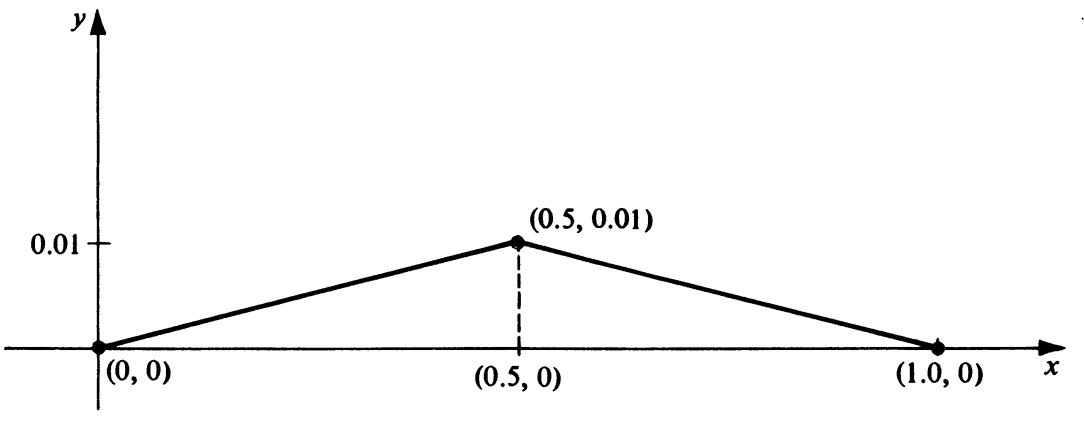
\includegraphics[width=0.75\textwidth]{figure/1_page_2.PNG}
		\caption*{Figure 14.2}\label{fig14.2}
	\end{figure}
	%
\end{document}